\documentclass{standalone}
\usepackage{tikz}
\usetikzlibrary{patterns}
\usetikzlibrary{positioning}
\usetikzlibrary{patterns, positioning}
\usetikzlibrary{shapes.misc}
\usepackage[outline]{contour}
\contourlength{1.5pt} 


\begin{document}
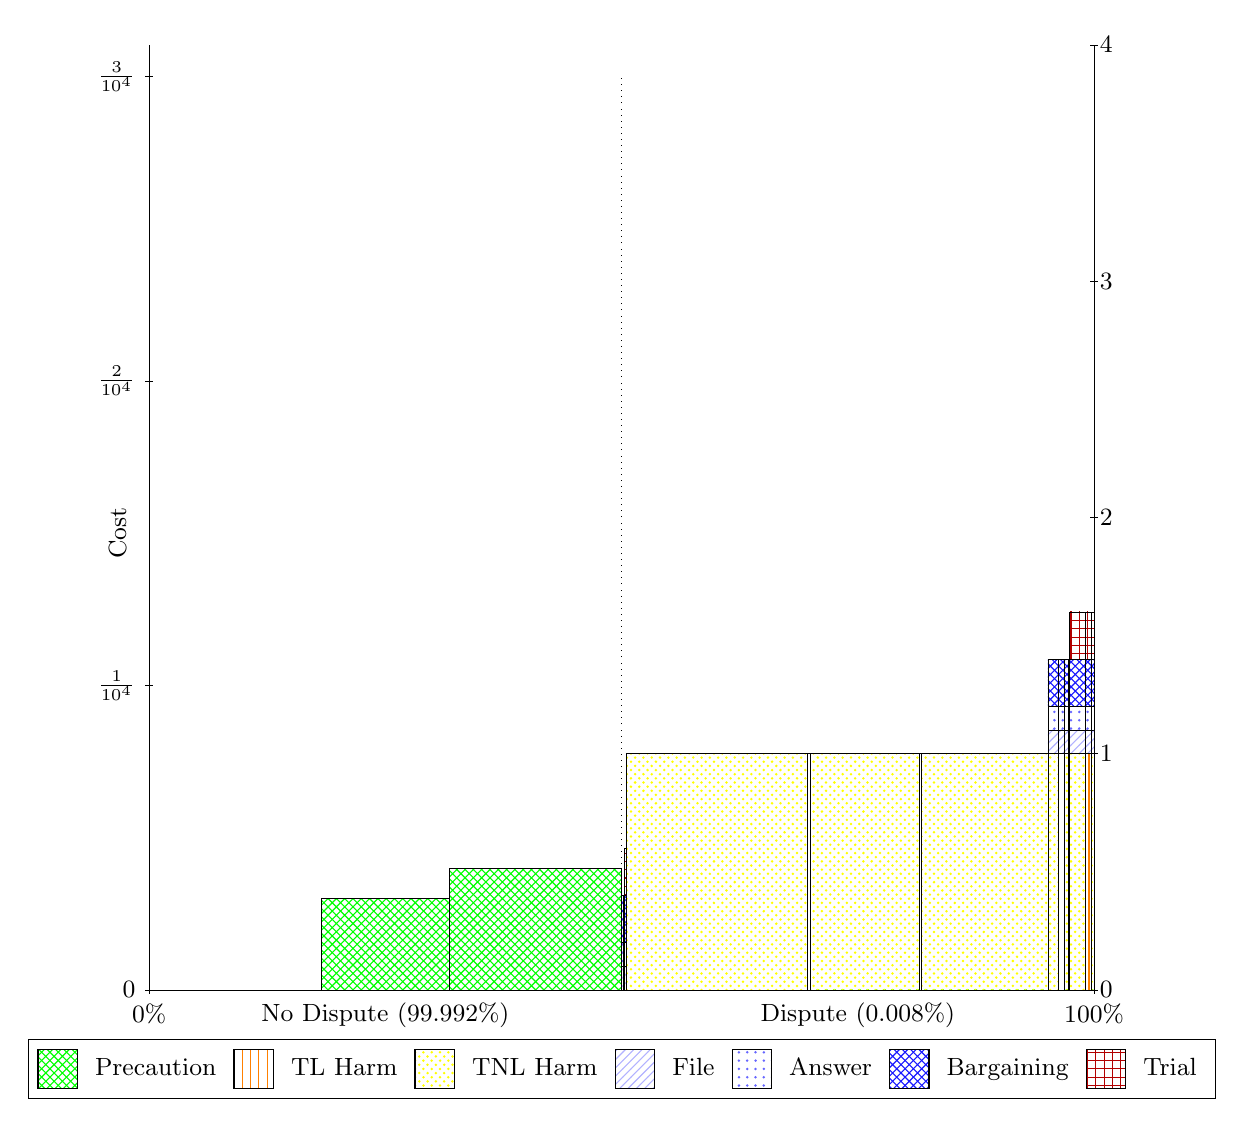
\begin{tikzpicture}
\draw[pattern=crosshatch, pattern color=green,draw=black,very thin] (3.6907,2.5) rectangle (5.3092,3.6598);
\draw[pattern=crosshatch, pattern color=green,draw=black,very thin] (5.3092,2.5) rectangle (7.5,4.0464);
\draw[pattern=north east lines, pattern color=blue!30,draw=black,very thin] (7.5,2.5) rectangle (7.5208,2.8);
\draw[pattern=dots,  pattern color=blue!60,draw=black,very thin] (7.5,2.8) rectangle (7.5208,3.1);
\draw[pattern=crosshatch,      pattern color=blue!90,draw=black,very thin] (7.5,3.1) rectangle (7.5208,3.7);
\draw[pattern=crosshatch, pattern color=green,draw=black,very thin] (7.5208,2.5) rectangle (7.5308,2.5001);
\draw[pattern=north east lines, pattern color=blue!30,draw=black,very thin] (7.5208,2.5001) rectangle (7.5308,2.8001);
\draw[pattern=dots,  pattern color=blue!60,draw=black,very thin] (7.5208,2.8001) rectangle (7.5308,3.1001);
\draw[pattern=crosshatch,      pattern color=blue!90,draw=black,very thin] (7.5208,3.1001) rectangle (7.5308,3.7001);
\draw[pattern=north east lines, pattern color=blue!30,draw=black,very thin] (7.5308,2.5) rectangle (7.5591,2.8);
\draw[pattern=dots,  pattern color=blue!60,draw=black,very thin] (7.5308,2.8) rectangle (7.5591,3.1);
\draw[pattern=crosshatch,      pattern color=blue!90,draw=black,very thin] (7.5308,3.1) rectangle (7.5591,3.7);
\draw[pattern=grid,            pattern color=red!70!black,draw=black,very thin] (7.5308,3.7) rectangle (7.5591,4.3);
\draw[pattern=crosshatch, pattern color=green,draw=black,very thin] (7.5591,2.5) rectangle (7.5639,2.5001);
\draw[pattern=north east lines, pattern color=blue!30,draw=black,very thin] (7.5591,2.5001) rectangle (7.5639,2.8001);
\draw[pattern=dots,  pattern color=blue!60,draw=black,very thin] (7.5591,2.8001) rectangle (7.5639,3.1001);
\draw[pattern=crosshatch,      pattern color=blue!90,draw=black,very thin] (7.5591,3.1001) rectangle (7.5639,3.7001);
\draw[pattern=grid,            pattern color=red!70!black,draw=black,very thin] (7.5591,3.7001) rectangle (7.5639,4.3001);
\draw[pattern=crosshatch dots, pattern color=yellow,draw=black,very thin] (7.5639,2.5) rectangle (9.8612,5.5);
\draw[pattern=vertical lines, pattern color=orange,draw=black,very thin] (9.8612,2.5) rectangle (9.8963,5.5);
\draw[pattern=crosshatch, pattern color=green,draw=black,very thin] (9.8963,2.5) rectangle (11.282,2.5001);
\draw[pattern=crosshatch dots, pattern color=yellow,draw=black,very thin] (9.8963,2.5001) rectangle (11.282,5.5001);
\draw[pattern=crosshatch, pattern color=green,draw=black,very thin] (11.282,2.5) rectangle (11.306,2.5001);
\draw[pattern=vertical lines, pattern color=orange,draw=black,very thin] (11.282,2.5001) rectangle (11.306,5.5001);
\draw[pattern=crosshatch, pattern color=green,draw=black,very thin] (11.306,2.5) rectangle (12.912,2.5001);
\draw[pattern=crosshatch dots, pattern color=yellow,draw=black,very thin] (11.306,2.5001) rectangle (12.912,5.5001);
\draw[pattern=crosshatch dots, pattern color=yellow,draw=black,very thin] (12.912,2.5) rectangle (13.046,5.5);
\draw[pattern=north east lines, pattern color=blue!30,draw=black,very thin] (12.912,5.5) rectangle (13.046,5.8);
\draw[pattern=dots,  pattern color=blue!60,draw=black,very thin] (12.912,5.8) rectangle (13.046,6.1);
\draw[pattern=crosshatch,      pattern color=blue!90,draw=black,very thin] (12.912,6.1) rectangle (13.046,6.7);
\draw[pattern=vertical lines, pattern color=orange,draw=black,very thin] (13.046,2.5) rectangle (13.12,5.5);
\draw[pattern=north east lines, pattern color=blue!30,draw=black,very thin] (13.046,5.5) rectangle (13.12,5.8);
\draw[pattern=dots,  pattern color=blue!60,draw=black,very thin] (13.046,5.8) rectangle (13.12,6.1);
\draw[pattern=crosshatch,      pattern color=blue!90,draw=black,very thin] (13.046,6.1) rectangle (13.12,6.7);
\draw[pattern=crosshatch, pattern color=green,draw=black,very thin] (13.12,2.5) rectangle (13.166,2.5001);
\draw[pattern=crosshatch dots, pattern color=yellow,draw=black,very thin] (13.12,2.5001) rectangle (13.166,5.5001);
\draw[pattern=north east lines, pattern color=blue!30,draw=black,very thin] (13.12,5.5001) rectangle (13.166,5.8001);
\draw[pattern=dots,  pattern color=blue!60,draw=black,very thin] (13.12,5.8001) rectangle (13.166,6.1001);
\draw[pattern=crosshatch,      pattern color=blue!90,draw=black,very thin] (13.12,6.1001) rectangle (13.166,6.7001);
\draw[pattern=crosshatch, pattern color=green,draw=black,very thin] (13.166,2.5) rectangle (13.185,2.5001);
\draw[pattern=vertical lines, pattern color=orange,draw=black,very thin] (13.166,2.5001) rectangle (13.185,5.5001);
\draw[pattern=north east lines, pattern color=blue!30,draw=black,very thin] (13.166,5.5001) rectangle (13.185,5.8001);
\draw[pattern=dots,  pattern color=blue!60,draw=black,very thin] (13.166,5.8001) rectangle (13.185,6.1001);
\draw[pattern=crosshatch,      pattern color=blue!90,draw=black,very thin] (13.166,6.1001) rectangle (13.185,6.7001);
\draw[pattern=crosshatch dots, pattern color=yellow,draw=black,very thin] (13.185,2.5) rectangle (13.382,5.5);
\draw[pattern=north east lines, pattern color=blue!30,draw=black,very thin] (13.185,5.5) rectangle (13.382,5.8);
\draw[pattern=dots,  pattern color=blue!60,draw=black,very thin] (13.185,5.8) rectangle (13.382,6.1);
\draw[pattern=crosshatch,      pattern color=blue!90,draw=black,very thin] (13.185,6.1) rectangle (13.382,6.7);
\draw[pattern=grid,            pattern color=red!70!black,draw=black,very thin] (13.185,6.7) rectangle (13.382,7.3);
\draw[pattern=vertical lines, pattern color=orange,draw=black,very thin] (13.382,2.5) rectangle (13.468,5.5);
\draw[pattern=north east lines, pattern color=blue!30,draw=black,very thin] (13.382,5.5) rectangle (13.468,5.8);
\draw[pattern=dots,  pattern color=blue!60,draw=black,very thin] (13.382,5.8) rectangle (13.468,6.1);
\draw[pattern=crosshatch,      pattern color=blue!90,draw=black,very thin] (13.382,6.1) rectangle (13.468,6.7);
\draw[pattern=grid,            pattern color=red!70!black,draw=black,very thin] (13.382,6.7) rectangle (13.468,7.3);
\draw[pattern=crosshatch, pattern color=green,draw=black,very thin] (13.468,2.5) rectangle (13.496,2.5001);
\draw[pattern=crosshatch dots, pattern color=yellow,draw=black,very thin] (13.468,2.5001) rectangle (13.496,5.5001);
\draw[pattern=north east lines, pattern color=blue!30,draw=black,very thin] (13.468,5.5001) rectangle (13.496,5.8001);
\draw[pattern=dots,  pattern color=blue!60,draw=black,very thin] (13.468,5.8001) rectangle (13.496,6.1001);
\draw[pattern=crosshatch,      pattern color=blue!90,draw=black,very thin] (13.468,6.1001) rectangle (13.496,6.7001);
\draw[pattern=grid,            pattern color=red!70!black,draw=black,very thin] (13.468,6.7001) rectangle (13.496,7.3001);
\draw[pattern=crosshatch, pattern color=green,draw=black,very thin] (13.496,2.5) rectangle (13.5,2.5001);
\draw[pattern=vertical lines, pattern color=orange,draw=black,very thin] (13.496,2.5001) rectangle (13.5,5.5001);
\draw[pattern=north east lines, pattern color=blue!30,draw=black,very thin] (13.496,5.5001) rectangle (13.5,5.8001);
\draw[pattern=dots,  pattern color=blue!60,draw=black,very thin] (13.496,5.8001) rectangle (13.5,6.1001);
\draw[pattern=crosshatch,      pattern color=blue!90,draw=black,very thin] (13.496,6.1001) rectangle (13.5,6.7001);
\draw[pattern=grid,            pattern color=red!70!black,draw=black,very thin] (13.496,6.7001) rectangle (13.5,7.3001);
\draw[black,very thin] (1.5,2.5) -- (1.5,14.5);
\node[font=\small,rotate=90,text=black, anchor=center] at (1.1, 8.2988) {Cost};
\draw[black,very thin] (1.45,2.5) -- (1.55,2.5);
\node[font=\small,text=black, anchor=east] at (1.45, 2.5) {0};
\draw[black,very thin] (1.45,6.3659) -- (1.55,6.3659);
\node[font=\small,text=black, anchor=east] at (1.45, 6.3659) {$\frac{1}{10^{4}}$};
\draw[black,very thin] (1.45,10.232) -- (1.55,10.232);
\node[font=\small,text=black, anchor=east] at (1.45, 10.232) {$\frac{2}{10^{4}}$};
\draw[black,very thin] (1.45,14.098) -- (1.55,14.098);
\node[font=\small,text=black, anchor=east] at (1.45, 14.098) {$\frac{3}{10^{4}}$};

\draw[black,dotted,very thin] (7.5,2.86) -- (7.5,14.14);
\draw[black,very thin] (13.5,2.5) -- (13.5,14.5);
\draw[black,very thin] (13.45,2.5) -- (13.55,2.5);
\node[font=\small,text=black, anchor=west] at (13.45, 2.5) {0};
\draw[black,very thin] (13.45,5.5) -- (13.55,5.5);
\node[font=\small,text=black, anchor=west] at (13.45, 5.5) {1};
\draw[black,very thin] (13.45,8.5) -- (13.55,8.5);
\node[font=\small,text=black, anchor=west] at (13.45, 8.5) {2};
\draw[black,very thin] (13.45,11.5) -- (13.55,11.5);
\node[font=\small,text=black, anchor=west] at (13.45, 11.5) {3};
\draw[black,very thin] (13.45,14.5) -- (13.55,14.5);
\node[font=\small,text=black, anchor=west] at (13.45, 14.5) {4};

\draw[black,very thin] (1.5,2.5) -- (13.5,2.5);
\draw[black,very thin] (1.5,2.45) -- (1.5,2.55);
\node[font=\small,text=black, anchor=north] at (1.5, 2.45) {0\%};
\draw[black,very thin] (13.5,2.45) -- (13.5,2.55);
\node[font=\small,text=black, anchor=north] at (13.5, 2.45) {100\%};

\node[font=\small,text=black,anchor=south] at (4.5, 1.9) {No\ Dispute\ (99.992\%)};
\node[font=\small,text=black,anchor=south] at (10.5, 1.9) {Dispute\ (0.008\%)};
\draw (7.5,2.5) node (B) {};
\begin{scope}[align=center]
\matrix[scale=0.5,draw=black,below=0.5cm of B,nodes={draw},column sep=0.1cm]{
\node[rectangle,draw,minimum width=0.5cm,minimum height=0.5cm,pattern=crosshatch, pattern color=green]{}; & \node[draw=none,font=\small,text=black]{Precaution}; &
\node[rectangle,draw,minimum width=0.5cm,minimum height=0.5cm,pattern=vertical lines, pattern color=orange]{}; & \node[draw=none,font=\small,text=black]{TL Harm}; &
\node[rectangle,draw,minimum width=0.5cm,minimum height=0.5cm,pattern=crosshatch dots, pattern color=yellow]{}; & \node[draw=none,font=\small,text=black]{TNL Harm}; &
\node[rectangle,draw,minimum width=0.5cm,minimum height=0.5cm,pattern=north east lines, pattern color=blue!30]{}; & \node[draw=none,font=\small,text=black]{File}; &
\node[rectangle,draw,minimum width=0.5cm,minimum height=0.5cm,pattern=dots,  pattern color=blue!60]{}; & \node[draw=none,font=\small,text=black]{Answer}; &
\node[rectangle,draw,minimum width=0.5cm,minimum height=0.5cm,pattern=crosshatch,      pattern color=blue!90]{}; & \node[draw=none,font=\small,text=black]{Bargaining}; &
\node[rectangle,draw,minimum width=0.5cm,minimum height=0.5cm,pattern=grid,            pattern color=red!70!black]{}; & \node[draw=none,font=\small,text=black]{Trial}; \\\\
};\end{scope}

\end{tikzpicture}
\end{document}